\subsection{Kinds of Models}
\begin{frame}{Kinds of Models}
    \framesubtitle{Vocabularies and Constraints}


    \AddToShipoutPictureFG*{
    \AtPageUpperLeft{\put(-5,-15){\makebox[\paperwidth][r]{Requirement 1}}}
    }%

        \begin{table}[]
            \begin{tabular}{ccc}
                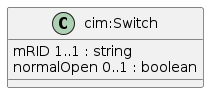
\includegraphics[width=0.3\textwidth]{slides/kinds/switches-examples/figs/switch1.png}& 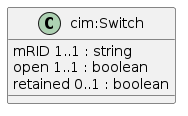
\includegraphics[width=0.3\textwidth]{slides/kinds/switches-examples/figs/switch2.png} & 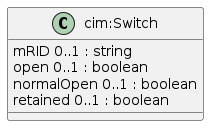
\includegraphics[width=0.3\textwidth]{slides/kinds/switches-examples/figs/SwitchVocab.png} \\
            \multicolumn{1}{l}{}                                                        & \multicolumn{1}{l}{}                                                                 & \multicolumn{1}{l}{}                                                          \\
            \begin{tabular}[c]{@{}c@{}}a Switch class with \\ 2 attributes\end{tabular} & \begin{tabular}[c]{@{}c@{}}a Switch class with\\ 2 different attributes\end{tabular} & \begin{tabular}[c]{@{}c@{}}a Switch class with \\ all attributes\end{tabular} \\
            some compulsory                                                             & some compulsory                                                                      & all optional                                                                
            \end{tabular}
        \end{table}
\end{frame}
